% !TeX document-id = {4b20f74a-885a-4146-b1bb-cebfdf55358e}
% !TeX program=lualatex
% !TeX TXS-program:bibliography=txs:///biber


% ========
% Preamble
% ========

% -----
% Class
% -----
\documentclass{bredelebeamer}

% ------------
% Slide layout
% ------------
\setbeamersize{%
  text margin left=0.3cm,%
  text margin right=0.3cm
}
%\usepackage{ragged2e}

\usepackage{appendixnumberbeamer}

% List spacing (enumitem is not compatible with beamer)
% https://jayrobwilliams.com/posts/2019/10/better-beamer
% https://tex.stackexchange.com/questions/369504#369597
\makeatletter
\renewcommand{\itemize}[1][]{%
  \beamer@ifempty{#1}{}{\def\beamer@defaultospec{#1}}%
  \ifnum \@itemdepth >2\relax\@toodeep\else
    \advance\@itemdepth\@ne
    \beamer@computepref\@itemdepth% sets \beameritemnestingprefix
    \usebeamerfont{itemize/enumerate \beameritemnestingprefix body}%
    \usebeamercolor[fg]{itemize/enumerate \beameritemnestingprefix body}%
    \usebeamertemplate{itemize/enumerate \beameritemnestingprefix body begin}%
    \list
    {\usebeamertemplate{itemize \beameritemnestingprefix item}}
    {\def\makelabel##1{%
        {%
          \hss\llap{{%
              \usebeamerfont*{itemize \beameritemnestingprefix item}%
              \usebeamercolor[fg]{itemize \beameritemnestingprefix item}##1}}%
        }%
      }%
    }
  \fi%
  \setlength\itemsep{\fill}
  \ifnum \@itemdepth >1
    \vfill
  \fi%
  \beamer@cramped%
  \raggedright%
  \beamer@firstlineitemizeunskip%
}
\def\enditemize{\ifhmode\unskip\fi\endlist%
  \usebeamertemplate{itemize/enumerate \beameritemnestingprefix body end}
  \ifnum \@itemdepth >1
  \vfil
  \fi%
}
\makeatother

\makeatletter
\def\enumerate{%
  \ifnum\@enumdepth>2\relax\@toodeep
  \else%
  \advance\@enumdepth\@ne%
  \edef\@enumctr{enum\romannumeral\the\@enumdepth}%
  \advance\@itemdepth\@ne%
  \fi%
  \beamer@computepref\@enumdepth% sets \beameritemnestingprefix
  \edef\beamer@enumtempl{enumerate \beameritemnestingprefix item}%
  \@ifnextchar[{\beamer@@enum@}{\beamer@enum@}}
\def\beamer@@enum@[{\@ifnextchar<{\beamer@enumdefault[}{\beamer@@@enum@[}}
\def\beamer@enumdefault[#1]{\def\beamer@defaultospec{#1}%
  \@ifnextchar[{\beamer@@@enum@}{\beamer@enum@}}
\def\beamer@@@enum@[#1]{% partly copied from enumerate.sty
  \@enLab{}\let\@enThe\@enQmark
  \@enloop#1\@enum@
  \ifx\@enThe\@enQmark\@warning{The counter will not be printed.%
    ^^J\space\@spaces\@spaces\@spaces The label is: \the\@enLab}\fi
  \def\insertenumlabel{\the\@enLab}
  \def\beamer@enumtempl{enumerate mini template}%
  \expandafter\let\csname the\@enumctr\endcsname\@enThe
  \csname c@\@enumctr\endcsname7
  \expandafter\settowidth
  \csname leftmargin\romannumeral\@enumdepth\endcsname
  {\the\@enLab\hspace{\labelsep}}%
  \beamer@enum@}
\def\beamer@enum@{%
  \beamer@computepref\@itemdepth% sets \beameritemnestingprefix
  \usebeamerfont{itemize/enumerate \beameritemnestingprefix body}%
  \usebeamercolor[fg]{itemize/enumerate \beameritemnestingprefix body}%
  \usebeamertemplate{itemize/enumerate \beameritemnestingprefix body begin}%
  \expandafter
  \list
  {\usebeamertemplate{\beamer@enumtempl}}
  {\usecounter\@enumctr%
    \def\makelabel##1{{\hss\llap{{%
            \usebeamerfont*{enumerate \beameritemnestingprefix item}%
            \usebeamercolor[fg]{enumerate \beameritemnestingprefix item}##1}}}}}%
  \setlength\itemsep{\fill}
  \ifnum \@itemdepth >1
  \vfill
  \fi%
  \beamer@cramped%
  \raggedright%
  \beamer@firstlineitemizeunskip%
}
\def\endenumerate{\ifhmode\unskip\fi\endlist%
  \usebeamertemplate{itemize/enumerate \beameritemnestingprefix body end}
  \ifnum \@itemdepth >1
  \vfil
  \fi%
}
\makeatother

% Section title page
\AtBeginSection[]{
  \begin{frame}
  \vfill
  \centering
  \begin{beamercolorbox}[sep=8pt, center, shadow=true, rounded=true]{title}
    \usebeamerfont{title}\insertsectionhead\par%
  \end{beamercolorbox}
  \vfill
  \end{frame}
}

% Item icon
% Itemize
\setbeamertemplate{enumerate item}[square]
\setbeamertemplate{itemize item}{\raise0.1ex \hbox{\scriptsize\faAtom}}
\setbeamertemplate{itemize subitem}{\raise0.15ex \hbox{\tiny\faDiceD20}}
\setbeamertemplate{itemize subsubitem}{\raise0.1ex \hbox{\tiny\faCog}}

% -------------
% Maths support
% -------------
% Load maths packages
%% Typical packages
\usepackage{%
  amsmath,%
  amsthm,%
  amssymb,%
  mathrsfs,%
  mathtools,%
  gensymb,%
  braket,%
  mleftright,%
  nicefrac,%
  interval,%
  empheq,% for boxing aligned equations
  stmaryrd,% for double-lined brackets
  accents,% for accent fine-tuning
}

% Settings for packages
%% interval: change open fences to round brackets
\intervalconfig{soft open fences}

%% mleftright: redefine \left as \mleft and \right as \mright
\mleftright


% ------------------
% Scientific support
% ------------------
% Chemistry
\usepackage[version=4]{mhchem}

% Scientific typesetting
\usepackage{siunitx}


% ----------
% Typography
% ----------
% Context-sensitive quotation marks
\usepackage[english=british]{csquotes}

%% Micro-typography
%\usepackage[%
%  activate={true, nocompatibility},%
%  draft,%
%  tracking=true,%
%  factor=1100,%
%%  stretch=10,%
%%  shrink=10%
%]{microtype}
%
%% Reduce spacing between sc characters
%\SetTracking{encoding={*}, shape=sc}{40}


% -------------------
% Font configurations
% -------------------
% Font support
\usepackage[no-math]{fontspec}
\defaultfontfeatures{%
  Ligatures=TeX,%
  Numbers=Lining,%
}

\newfontfamily\Raleway{Raleway}[%
  UprightFont=*-Regular,%
  ItalicFont=*-Italic,%
  BoldFont=*-Bold,%
  BoldItalicFont=*-BoldItalic,%
  Ligatures=TeX,%
]
\newfontfamily\Lato{Lato}[%
  Ligatures=TeX,%
]

\usefonttheme{structurebold}

% Main font selection

\setmainfont{Lato}[%
  UprightFont=*-Regular,%
  ItalicFont=*-Italic,%
  BoldFont=*-Bold,%
  BoldItalicFont=*-BoldItalic,%
  Ligatures=TeX,%
]
\setsansfont{Lato}[%
  UprightFont=*-Regular,%
  ItalicFont=*-Italic,%
  BoldFont=*-Bold,%
  BoldItalicFont=*-BoldItalic,%
  Ligatures=TeX,%
]

\setbeamerfont{headline}{family=\Raleway}
\setbeamerfont{headline title}{size=\huge, series=\bfseries}
\setbeamerfont{headline author}{size=\Large}
\setbeamerfont{headline institute}{size=\normalsize}
\setbeamerfont{footline}{family=\Raleway}
\setbeamerfont{footline address}{size=\normalsize}
\setbeamerfont{block title}{family=\Raleway, size=\LARGE, series=\bfseries}
\setbeamerfont{block body}{size=\large}
\setbeamerfont{heading}{family=\Lato, series=\bfseries}
\setbeamerfont{caption}{size=\small}

\usepackage{fontawesome5}

% Maths font selection
\usepackage[%
  math-style=ISO,%
  bold-style=ISO,%
  warnings-off={mathtools-colon},%
]{unicode-math}

% Main maths font
\setmathfont{Fira Math}

% Missing glyph ranges
\setmathfont{STIX Two Math}[%
  range={cal, bfcal, sfup, frak, bffrak},%
]
\setmathfont{STIX Two Math}[%
  range={scr, bfscr}, StylisticSet=1,%
]

% ----------------
% Language support
% ----------------
% polyglossia requires fontspec
\usepackage{polyglossia}
\setmainlanguage[variant=british]{english}

% Date and time format
\usepackage{datetime}
\newdateformat{monthyeardate}{%
  \monthname[\THEMONTH] \THEYEAR
}


% -------
% Colours
% -------
% Colour aliases
\colorlet{SpinColour}{DarkGreen}
\colorlet{SpatialColour}{DeepPink3}


% ------
% Tables
% ------
\usepackage{booktabs, multirow}


% --------
% Diagrams
% --------
% Graphics
\usepackage{graphicx, transparent}
\usepackage[export]{adjustbox}

% TikZ & PGFPlots
\usepackage{pgfplots}

\pgfplotsset{compat=1.17}

\usetikzlibrary{%
  external,%
  calc,%
  luamath,%
  positioning,%
  decorations.pathreplacing,%
  arrows.meta,%
  3d,%
  backgrounds,%
  overlay-beamer-styles,%
  patterns,%
  spy,%
}

\usepgfplotslibrary{%
  groupplots,%
  patchplots,%
  colormaps,%
  fillbetween,%
}

% PGFPlots cycle colours
\pgfplotscreateplotcyclelist{coloronly}{%
  {red},%
  {blue},%
  {black!60!green},%
  {black!20!orange},%
  {green!30!brown},%
  {blue!40!red},%
  {black!60!blue},%
  {black!40!yellow},%
  {red!50!pink},%
  {green!70!blue},%
}

% TikZ styles
\tikzset{
  nodeStyleGreen/.style={
    draw=Tikzgreen,
    fill=Tikzgreenlight,
    align=left,
    thick,
    rounded corners
  }
}

\tikzset{
  nodeStyleRed/.style={
    draw=Tikzred,
    fill=Tikzredlight,
    align=left,\right)
    thick,
    rounded corners
  }
}

\tikzset{
  nodeStyleBlue/.style={
    draw=Tikzblue,
    fill=Tikzbluelight,
    align=left,
    thick,
    rounded corners
  }
}

\tikzset{
  lineStyleRed/.style={
    color=Tikzred,
    opacity=0.75,
    line width=2pt,
  }
}

\tikzset{
  lineStyleGreen/.style={
    color=Tikzgreen,
    opacity=0.75,
    line width=2pt,
  }
}

\tikzset{
  lineStyleBlue/.style={
    color=Tikzblue,
    opacity=0.75,
    line width=2pt,
  }
}

\def\MarkLt{6pt}
\def\MarkSep{3pt}
\tikzset{
  TwoMarks/.style={
    postaction={
      decorate,
      decoration={
        markings,
        mark=at position #1 with{
          \begin{scope}[xslant=0.2]
            \draw[line width=\MarkSep,white,-] (0pt,-\MarkLt) -- (0pt,\MarkLt);
            \draw[-] (-0.5*\MarkSep,-\MarkLt) -- (-0.5*\MarkSep,\MarkLt);
            \draw[-] (0.5*\MarkSep,-\MarkLt) -- (0.5*\MarkSep,\MarkLt);
          \end{scope}
        }
      }
    }
  },
  TwoMarks/.default={0.5}
}

% Plot conditionals
\usepackage{xifthen}

% Equation highlighting
\usepackage[customcolors, beamer, markings]{hf-tikz}

% TikZ externalize switch
\newif\iftikzex
%\tikzextrue
\tikzexfalse

% Command for tikzexternalize/includegraphics
\tikzexternalize
\makeatletter
\newcommand*{\useexternalfile}[4]{
  \iftikzex
    \tikzsetnextfilename{tikzoutput/#4-output}
    \scalebox{#1}{\input{\tikzexternal@filenameprefix#4.tikz.tex}}
  \else
    \includegraphics[scale=#1, trim=#2 0 #3 0]{\tikzexternal@filenameprefix tikzoutput/#4-output.pdf}
  \fi
}
\makeatother
\tikzexternaldisable

% Subplots
\usepackage{subcaption}


% ----------
% Animations
% ----------
\usepackage[final, controls, buttonsize=0.8em]{animate}


% ------------------------
% References & bookmarking
% ------------------------
% Hyperlink references
\usepackage{hyperref}

% Footnotes
\renewcommand{\thefootnote}{\alph{footnote}}

% Footnote kerning with punctuation
% Do not use with option multiple for footmisc since this package has a different way of handling multiple footnotes.
\usepackage{fnpct}

% Bibliography
\usepackage[
  sorting=none,
  giveninits=true,
  style=nature,
  autocite=superscript,
  dateabbrev=false,
  doi=false,
  url=false,
  isbn=false,
  backend=biber
]{biblatex}
\addbibresource{bib/magic-sep2022.bib}

\newrobustcmd*{\footlessfullcite}{
  \AtNextCite{
    \renewbibmacro{title}{}\renewbibmacro{in:}{}
  }
  \footfullcite
}
\makeatletter
  \def\@makefnmark{}
\makeatletter
\AtEveryCitekey{\iffootnote{\tiny}{\footnotesize}}

\renewbibmacro*{name:andothers}{% Based on name:andothers from biblatex.def
  \ifboolexpr{
    test {\ifnumequal{\value{listcount}}{\value{liststop}}}
    and
    test \ifmorenames
  }
  {\ifnumgreater{\value{liststop}}{1}
     {\finalandcomma}
     {}%
   \andothersdelim\bibstring[\textit]{andothers}}
  {}%
}

\setlength{\footnotesep}{2pt}
\addtobeamertemplate{footnote}{\hskip -1.7em}{}


% -----------------
% Cross-referencing
% -----------------
% To be loaded after hyperref
\usepackage[capitalise, noabbrev]{cleveref}


% --------------------------
% Special symbols & commands
% --------------------------
% Symbols
\newcommand*{\D}{\mathrm{d}}
\newcommand*{\euler}{e}
\newcommand*{\imag}{i}
\newcommand*{\T}{\symsfup{T}}

% Commands
\newcommand*{\vecop}[1]{\hat{\boldsymbol{#1}}}
\newcommand*{\norm}[1]{\left\lVert#1\right\rVert}
\newcommand*{\emphbf}[2]{%
  \textbf{\color{#1}#2}%
}
\newcommand*{\emphit}[2]{%
  \textit{\color{#1} #2}%
}
\newcommand*\widefbox[1]{\fbox{\hspace{1em}#1\hspace{1em}}}

% Operators
\DeclareMathOperator{\Tr}{tr}
\DeclareMathOperator{\Ln}{Ln}
\DeclareMathOperator{\id}{id}
\DeclareMathOperator{\diag}{diag}
\DeclareMathOperator*{\argmin}{argmin}
\DeclareMathOperator*{\re}{\symfrak{Re}}


%% Latin abbreviations
\usepackage{xspace}
\newcommand*{\eg}{\textit{e.g.}\@\xspace}
\newcommand*{\ie}{\textit{i.e.}\@\xspace}
\newcommand*{\ca}{\textit{ca.}\@\xspace}
\newcommand*{\cf}{\textit{cf.}\@\xspace}

\makeatletter
\newcommand*{\etc}{%
    \@ifnextchar{.}%
        {\textit{etc}}%
        {\textit{etc}.\@\xspace}%
}
\makeatother

% New commands
\makeatletter
\newcommand{\annotate}[5]{
  % Format: \annotate{overlay scope}{colour}{path}{alignment}{text}
  \begin{tikzpicture}[overlay]
    \draw<#1>[stealth-, #2, draw, use marker id] #3 node[#4]{#5};
  \end{tikzpicture}
}

\newcommand*\bigcdot{
  \mathpalette\bigcdot@{.5}
}
\newcommand*\bigcdot@[2]{
  \mathbin{
    \vcenter{
      \hbox{\scalebox{#2}{$\m@th#1\bullet$}}
    }
  }
}
\makeatother

% List of symbols
\usepackage[%
  nonumberlist,%
  symbols,%
  nogroupskip,%
  nopostdot,%
  nohypertypes={symbols}
]{glossaries-extra} % package for glossaries


% Hyphenated long forms
\glsaddkey
  {hyphenated}        % new key
  {\relax}            % default value if "hyphenated" isn't used in \newglossaryentry
  {\glsentryhyphx}    % analogous to \glsentrytext
  {\Glsentryhyphx}    % analogous to \Glsentrytext
  {\glshyphx}         % analogous to \glstext
  {\Glshyphx}         % analogous to \Glstext
  {\GLShyphx}         % analogous to \GLStext
\newcommand{\GENglspostlinkhook}{%
  \ifglsused{\glslabel}{}{ (\glsentryshort{\glslabel})}\glsunset \glslabel}
\makeatletter
\newcommand\metadef[1]{%
  \expandafter\newcommand\csname gls#1\endcsname{%
    \@ifstar{\csname sgls#1\endcsname}{\csname ngls#1\endcsname}%
  }
  \@namedef{sgls#1}##1{{\let\glspostlinkhook \GENglspostlinkhook\expandafter\csname gls#1x\endcsname*{##1}}}%
  \@namedef{ngls#1}##1{{\let\glspostlinkhook \GENglspostlinkhook\expandafter\csname gls#1x\endcsname{##1}}}%
  \expandafter\newcommand\csname Gls#1\endcsname{%
    \@ifstar{\csname sGls#1\endcsname}{\csname nGls#1\endcsname}%
  }
  \@namedef{sGls#1}##1{{\let\glspostlinkhook \GENglspostlinkhook\expandafter\csname Gls#1x\endcsname*{##1}}}%
  \@namedef{nGls#1}##1{{\let\glspostlinkhook \GENglspostlinkhook\expandafter\csname Gls#1x\endcsname{##1}}}%
  \expandafter\newcommand\csname GLS#1\endcsname{%
    \@ifstar{\csname sGLS#1\endcsname}{\csname nGLS#1\endcsname}%
  }
  \@namedef{sGLS#1}##1{{\let\glspostlinkhook \GENglspostlinkhook\expandafter\csname GLS#1x\endcsname*{##1}}}%
  \@namedef{nGLS#1}##1{{\let\glspostlinkhook \GENglspostlinkhook\expandafter\csname GLS#1x\endcsname{##1}}}%
}
\makeatother

\metadef{hyph}

\loadglsentries{symbols/symbols}
\loadglsentries{symbols/acronyms}

\makeatletter
% Thanks to Paul Gaborit https://tex.stackexchange.com/a/179946/38080
\def\extractcoord#1#2#3{
  \path let \p1=(#3) in \pgfextra{
    \pgfmathsetmacro#1{\x{1}/\pgf@xx}
    \pgfmathsetmacro#2{\y{1}/\pgf@yy}
    \xdef#1{#1} \xdef#2{#2}
  };
}
\makeatother
\newcommand{\showboundingbox}{%
    %
    % Show the bounding box of the tikzpicture. Use as last command.
    % It will not change the bounding box thanks to the overlay option.
    %
    \extractcoord\xa\ya{current bounding box.south west}
    \extractcoord\xb\yb{current bounding box.north east}
    \node [overlay, draw=red, fill=white, opacity=0.8, font=\tiny\ttfamily, anchor=north east] at (current bounding box.north east) {(\xa, \ya) (\xb, \yb)};
}

% ---------------
% Special lengths
% ---------------
\newlength{\size}
\setlength{\size}{0.6cm}
\newlength{\marksize}
\newlength{\plotheight}
\newlength{\plotwidth}

% -----
% Title
% -----
\title[Symmetry of MAGIC]{Symmetry of Magnetically Induced Currents}

\subtitle{
  {\small \normalfont \textit{MAGIC 2022 | Peterhouse, Cambridge, UK}}
}

\author[\underline{B. C. Huynh}, A. M. Teale]{\underline{Bang C. Huynh}\inst{\tiny $\dagger$}, Andrew M. Teale\inst{\tiny $\dagger$}}

\institute[]{
  \inst{\tiny $\dagger$}School of Chemistry, University of Nottingham, UK
}

\date[13th September 2022]{13\textsuperscript{\tiny th} September 2022}


\titlegraphic{
  
\includegraphics[height=0.7cm, keepaspectratio]{images/UoNlogo.eps}
  \hspace{0.5cm}
  
\includegraphics[height=0.7cm, keepaspectratio]{images/LOGO_ERC.eps}
  \hspace{0.5cm}
  
\includegraphics[height=0.7cm, keepaspectratio]{images/quest.eps}

  \vspace{0.5cm}

  
\includegraphics[height=0.7cm, keepaspectratio]{images/Peterhouse_shield.eps}
  \hspace{0.5cm}
  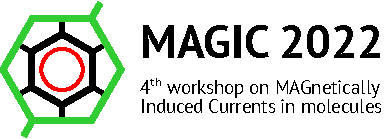
\includegraphics[height=0.7cm, keepaspectratio]{images/magic_logo/magiclogo.pdf}
}


% ----
% Main
% ----

%\includeonly{cursym/cursym}
%\includeonlyframes{current}
\begin{document}
% \tikzexternaldisable
  % For every picture that defines or uses external nodes, you'll have to apply the 'remember picture' style. To avoid some typing, we'll apply
  % the style to all pictures.
  \tikzstyle{every picture}+=[remember picture]

  % By default all math in TikZ nodes are set in inline mode. Change this to
  % displaystyle so that we don't get small fractions.
  \everymath{\displaystyle}

  %%%%%%%%%%%%%%%%%%%%%%%%%%%%%%%%%%%%%%%%%%%%%%%%%%%%%%%%
  %%%%%%%%%%%%%%%%%%%%%%%%%%%%%%%%%%%%%%%%%%%%%%%%%%%%%%%%
  \begin{frame}
    \titlepage
  \end{frame}
  %%%%%%%%%%%%%%%%%%%%%%%%%%%%%%%%%%%%%%%%%%%%%%%%%%%%%%%%
  %%%%%%%%%%%%%%%%%%%%%%%%%%%%%%%%%%%%%%%%%%%%%%%%%%%%%%%%

  \section{Introduction}

  %%%%%%%%%%%%%%%%%%%%%%%%%%
  %%%%%%%%%%%%%%%%%%%%%%%%%%
  \begin{frame}{Overview}
    \begin{itemize}
      \item Symmetry and pseudo-symmetry \emphit{Magenta}{groups} in magnetic fields
      \item \emphit{Magenta}{Unitary} representation analysis on \emphit{Magenta}{linear spaces}
      \item \emphit{Magenta}{Wavefunction} and \emphit{Magenta}{current density} symmetries
      \begin{itemize}
        \item \emphit{Magenta}{Relationships} between wavefunction and current density symmetries
        \item Symmetry \emphit{Magenta}{descent} and symmetry \emphit{Magenta}{breaking} in magnetic fields
      \end{itemize}
    \end{itemize}
  \end{frame}
  \section{Groups in magnetic fields}

  \subsection{Hamiltonian transformations}
  %%%%%%%%%%%%%%%%%%%%%%%%%%
  %%%%%%%%%%%%%%%%%%%%%%%%%%
  \begin{frame}{The electronic Hamiltonian}
    \begin{itemize}
      \item<1-> For an $\gls*{gen:Ne}$-electron system in a \emphit{Magenta}{uniform} magnetic field $\gls*{mag:vec} = \symbf{\nabla} \times \gls*{mag:vecpot}(\gls*{bas:spatialcoord})$, consider the \emphbf{DarkGreen}{Schr\"{o}dinger--Pauli Hamiltonian} in atomic units:
      \begin{align*}
        \gls*{op:hamil}
          &= \tikzmarkin<2>[nodeStyleGreen, mark at=0.82]{kin}(0.04,-0.60)(-0.06,0.80)
            \annotate{2}{red}{(0,0)--++(0,-0.3)}{below}{%
              kinetic%
            }
            \frac{1}{2}
            \sum_{k=1}^{\gls*{gen:Ne}}
            \left\lvert
              -\hat{\symbfit{p}}_k + \gls*{mag:vecpot}(\gls*{bas:spatialcoord}[_k])
            \right\rvert^2
          \tikzmarkend{kin}
          + \tikzmarkin<3>[nodeStyleGreen, mark at=0.85]{potex}(0.04,-0.60)(-0.06,0.80)
            \annotate{3}{red}{(0,0)--++(0,-0.3)}{below}{%
              external potential%
            }
            \sum_{k=1}^{\gls*{gen:Ne}}
              \gls*{op:pot1e}[_{\symup{ext}}](\gls*{bas:spatialcoord}[_k])
          \tikzmarkend{potex}
          + \tikzmarkin<4>[nodeStyleGreen, mark at=0.82]{ee}(0.04,-0.60)(-0.06,0.80)
            \annotate{4}{red}{(0,0)--++(0,-0.3)}{below}{%
              electron--electron interaction%
            }
            \frac{1}{2}
              \sum_{k \ne l}^{\gls*{gen:Ne}}
              \frac{1}{\lvert \gls*{bas:spatialcoord}[_k] - \gls*{bas:spatialcoord}[_l] \rvert}
          \tikzmarkend{ee}
          + \tikzmarkin<5>[nodeStyleGreen, mark at=0.845]{eb}(0.04,-0.60)(-0.06,0.80)
            \annotate{5}{red}{(0,0)--++(0,-0.3)}{below}{%
              spin Zeeman interaction%
            }
              \frac{g_s}{2}
              \sum_{k=1}^{\gls*{gen:Ne}}
              \gls*{mag:vec} \cdot \hat{\symbfit{s}}_k
          \tikzmarkend{eb}
          \\[6pt]
          \onslide<6->{
            &= \tikzmarkin<7>[nodeStyleGreen, mark at=0.795]{zerofieldhamil}(0.04,-0.60)(-0.06,0.80)
              \annotate{7}{red}{(0,0)--++(0,-0.3)}{below}{%
                Zero-field Hamiltonian, $\gls*{op:hamil}[_0](\gls*{op:pot1e}[_{\symup{ext}}])$%
              }
                \frac{1}{2} \sum_{k=1}^{\gls*{gen:Ne}} \hat{p}_k^2
                + \sum_{k=1}^{\gls*{gen:Ne}}
                  \gls*{op:pot1e}[_{\symup{ext}}](\gls*{bas:spatialcoord}[_k])
                + \frac{1}{2}
                  \sum_{k \ne l}^{\gls*{gen:Ne}}
                  \frac{1}{\lvert \gls*{bas:spatialcoord}[_k] - \gls*{bas:spatialcoord}[_l] \rvert}
              \tikzmarkend{zerofieldhamil}
              + \tikzmarkin<8>[nodeStyleGreen, mark at=0.815]{linearcontrib}(0.04,-0.60)(-0.06,0.80)
                \annotate{8}{red}{(0,0)--++(0,-0.3)}{below}{%
                  Linear%
                }
                  \gls*{mag:vecpot}(\gls*{bas:spatialcoord}[_k]) \cdot \hat{\symbfit{p}}_k
                  + \frac{g_s}{2}
                  \sum_{k=1}^{\gls*{gen:Ne}}
                  \gls*{mag:vec} \cdot \hat{\symbfit{s}}_k
              \tikzmarkend{linearcontrib}
              + \tikzmarkin<8>[nodeStyleGreen, mark at=0.86]{quadcontrib}(0.04,-0.60)(-0.06,0.80)
                \annotate{8}{red}{(0,0)--++(0,-0.3)}{below}{%
                  Quadratic%
                }
                  \frac{1}{2}A^2(\gls*{bas:spatialcoord}[_k])
              \tikzmarkend{quadcontrib}
          }
          \\[6pt]
          \onslide<9->{
            &= \gls*{op:hamil}[_0](\gls*{op:pot1e}[_{\symup{ext}}])
            + \gls*{mag:vecpot}(\gls*{bas:spatialcoord}[_k]) \cdot \hat{\symbfit{p}}_k
            + \frac{g_s}{2}
            \sum_{k=1}^{\gls*{gen:Ne}}
            \gls*{mag:vec} \cdot \hat{\symbfit{s}}_k
            + \frac{1}{2}A^2(\gls*{bas:spatialcoord}[_k]).
          }
      \end{align*}

      \item<9-> How does each term transform \emphit{red}{spatially} and \emphit{blue}{temporally}?
    \end{itemize}

    \footfullcite{book:Weil2007}
    \footlessfullcite{article:Tellgren2018}
    \footlessfullcite{article:Irons2021}
  \end{frame}


  %%%%%%%%%%%%%%%%%%%%%%%%%%
  %%%%%%%%%%%%%%%%%%%%%%%%%%
  \begin{frame}[t]{Tensor transformations}
    \begin{itemize}
      \item<1-> Let $\symbfit{v}$ be a rank-$k$ Cartesian tensor in three dimensions.
      \only<2-5>{
        \item<2-> \emphit{red}{Spatially}, let $u \in \symsfup{O}(3)$ be any \emphbf{DarkGreen}{proper} or \emphbf{DarkGreen}{improper rotation} that acts on an orthogonal basis $\{\symbfit{e}_i\}$ spanning $\symbb{R}^3$ according to
        \begin{equation*}
          \hat{u}\symbfit{e}_i =
            \symbfit{e}_j
            \ \tikzmarkin<3>[nodeStyleGreen, mark at=0.84]{urep}(0.04,-0.20)(-0.06,0.40)
              \annotate{3}{red}{(0,0)--++(0,-0.3)}{below}{%
                $\symbfit{U}$: representation matrix for $u$ in $\{\symbfit{e}_i\}$%
              }
                U_{ji}
            \tikzmarkend{urep}.
        \end{equation*}
        \onslide<4->{%
          To consider the \emphit{Magenta}{linear} action of $u$ on $\symbfit{v}$, let $\symbfit{v}' = \hat{u}\symbfit{v}$.
          \begin{itemize}
            \item<4-> $\symbfit{v}$ is a \emphbf{red}{polar} tensor if
            \begin{equation*}
              v'_{ab\ldots k} = U_{ap} U_{bq} \ldots U_{kz}\ v_{pq\ldots z}.
            \end{equation*}
            \item<4-> $\symbfit{v}$ is an \emphbf{red}{axial} tensor if
            \begin{equation*}
              v'_{ab\ldots k} =
                \tikzmarkin<5>[nodeStyleGreen, mark at=0.83]{udet}(0.04,-0.20)(-0.06,0.40)
                  \annotate{5}{red}{(0,0)--++(0,-0.3)}{below}{%
                    $+1$ for proper rotations, $-1$ for improper rotations%
                  }
                  \lvert\symbfit{U}\rvert
                \tikzmarkend{udet}
                U_{ap} U_{bq} \ldots U_{kz}\ v_{pq\ldots z}.
            \end{equation*}
          \end{itemize}%
        }%
      }
      \only<6-7>{
        \item<6-> \emphit{blue}{Temporally}, let $\gls*{op:timerevnohat}$ be the \emphbf{DarkGreen}{time reversal} that acts on an orthogonal basis $\{\gls*{bas:spinbasis}[_1], \gls*{bas:spinbasis}[_2]\}$ of a two-component spinor according to
        \begin{equation*}
          \gls*{op:timerev}
          \begin{bmatrix}
            \gls*{bas:spinbasis}[_1] & \gls*{bas:spinbasis}[_2]
          \end{bmatrix}
          = \begin{bmatrix*}[r]
            \gls*{bas:spinbasis}[^*_2] & -\gls*{bas:spinbasis}[^*_1]
          \end{bmatrix*}.
        \end{equation*}
        \onslide<7->{%
          To consider the \emphit{Magenta}{antilinear} action of $\gls*{op:timerevnohat}$ on $\symbfit{v}$, let $\symbfit{v}'' = \gls*{op:timerev}\symbfit{v}$.
          \begin{itemize}
            \item<7-> $\symbfit{v}$ is a \emphbf{blue}{time-even} tensor (\emphbf{blue}{$\symbfit{i}$}-tensor) if
            \begin{equation*}
              \symbfit{v}'' = \symbfit{v}.
            \end{equation*}
            \item<7-> $\symbfit{v}$ is a \emphbf{blue}{time-odd} tensor (\emphbf{blue}{$\symbfit{c}$}-tensor) if
            \begin{equation*}
              \symbfit{v}'' = -\symbfit{v}.
            \end{equation*}
          \end{itemize}
        }%
      }
    \end{itemize}

    \footfullcite{book:Birss1966}
    \footlessfullcite{article:Bradley1968}
    \footlessfullcite{bookchapter:Lazzeretti1993}
  \end{frame}


  %%%%%%%%%%%%%%%%%%%%%%%%%%
  %%%%%%%%%%%%%%%%%%%%%%%%%%
  \begin{frame}{Tensor classifications}
    \begin{itemize}
      \item<1-> There are \emphit{Magenta}{four} types of tensors under spatial-temporal transformations.
      \begin{columns}[T]
        \begin{column}{.45\textwidth}
          \begin{itemize}
            \item<1-> \emphbf{red}{polar} \emphbf{blue}{time-even} tensors
            \begin{itemize}
              \item position vectors $\gls*{bas:spatialcoord}$
            \end{itemize}
          \end{itemize}
        \end{column}
        \begin{column}{.45\textwidth}
          \begin{itemize}
            \item<1-> \emphbf{red}{polar} \emphbf{blue}{time-odd} tensors
            \begin{itemize}
              \item linear momentum vectors $\symbfit{p}$
              \item magnetic vector potentials $\gls*{mag:vecpot}$
              \item current densities $\gls*{mag:jphys}$
            \end{itemize}
          \end{itemize}
        \end{column}
      \end{columns}

      \vspace{0.2cm}

      \begin{columns}[T]
        \begin{column}{.45\textwidth}
          \begin{itemize}
            \item<1-> \emphbf{red}{axial} \emphbf{blue}{time-even} tensors
          \end{itemize}
        \end{column}
        \begin{column}{.45\textwidth}
          \begin{itemize}
            \item<1-> \emphbf{red}{axial} \emphbf{blue}{time-odd} tensors
            \begin{itemize}
              \item angular momentum vectors $\symbfit{l}$
              \item magnetic field vectors $\gls*{mag:vec}$
            \end{itemize}
          \end{itemize}
        \end{column}
      \end{columns}
    \end{itemize}

    \footfullcite{book:Birss1966}
    \footlessfullcite{article:Bradley1968}
    \footlessfullcite{bookchapter:Lazzeretti1993}
  \end{frame}


  \subsection{Hamiltonian invariance}
  %%%%%%%%%%%%%%%%%%%%%%%%%%
  %%%%%%%%%%%%%%%%%%%%%%%%%%
  \begin{frame}{Symmetry and pseudo-symmetry groups}
    \begin{itemize}
      \onslide<1->{
        \begin{alertblock}{Definition (symmetry group)}
          All transformations $\hat{T}$ that leave the electronic Hamiltonian $\gls*{op:hamil}$ invariant, \ie $\hat{T}\gls*{op:hamil}\hat{T}^{-1} = \gls*{op:hamil}$, form the \emphbf{DarkGreen}{symmetry group} of $\gls*{op:hamil}$.
          Such transformations are called \emphbf{DarkGreen}{symmetry transformations}.
        \end{alertblock}
      }
      \item<1-> Symmetry transformations impose \emphit{Magenta}{constraints} on the eigenfunctions of $\gls*{op:hamil}$ and properties calculated from them.\\[6pt]
      \onslide<2->{
        \begin{alertblock}{Definition (pseudo-symmetry group)}
          Consider a term $\gls*{op:hamil}' \subset \gls*{op:hamil}$.
          All transformations $\hat{T}$ that leave $\gls*{op:hamil}'$ invariant but not the full $\gls*{op:hamil}$ form a \emphbf{DarkGreen}{pseudo-symmetry group} of $\gls*{op:hamil}$.
          Such transformations are called \emphbf{DarkGreen}{pseudo-symmetry transformations}.
        \end{alertblock}
      }
      \item<2-> Pseudo-symmetry transformations provide ways to understand eigenfunctions of \emphit{Magenta}{$\gls*{op:hamil}$ (complicated)} from the perspective of \emphit{Magenta}{$\gls*{op:hamil}'$ (simpler)}.
    \end{itemize}
  \end{frame}


  %%%%%%%%%%%%%%%%%%%%%%%%%%
  %%%%%%%%%%%%%%%%%%%%%%%%%%
  \begin{frame}{Groups in magnetic fields}
    \begin{itemize}
      \item<1-> Let us revisit the electronic Hamiltonian in a uniform magnetic field:
      \begin{equation*}
        \gls*{op:hamil} =
          \tikzmarkin<2-3>[nodeStyleGreen, mark at=0.79]{zerofieldhamilgroup}(0.04,-0.20)(-0.06,0.40)
            \annotate{2-3}{red, align=center}{(0,0)--++(0,-0.3)}{below}{%
              \only<2>{\emphbf{red}{polar} \emphbf{blue}{time-even}\\}%
              \only<3>{\textcolor{DarkGreen}{$\symcal{G} + \gls*{op:timerevnohat} \symcal{G}$}}%
            }
            \gls*{op:hamil}[_0](\gls*{op:pot1e}[_{\symup{ext}}])
          \tikzmarkend{zerofieldhamilgroup}
          %%%
          + \tikzmarkin<6>[nodeStyleGreen, mark at=0.83]{Apgroup}(0.04,-0.40)(-0.06,0.60)
            \annotate{6}{red, align=center}{(0,0)--++(0,-0.3)}{below}{%
              \textcolor{DarkGoldenrod}{$\symsfup{O}(3) + \gls*{op:timerevnohat} \symsfup{O}(3)$}%
            }
            \tikzmarkin<4>[nodeStyleGreen, mark at=0.82]{Agroup}(0.04,-0.20)(-0.06,0.40)
              \annotate{4}{red, align=center}{(0,0)--++(0,-0.3)}{below}{%
                \emphbf{red}{polar} \emphbf{blue}{time-odd}%
              }
              \gls*{mag:vecpot}(\gls*{bas:spatialcoord}[_k])
            \tikzmarkend{Agroup}
            \cdot
            \tikzmarkin<5>[nodeStyleGreen, mark at=0.84]{pgroup}(0.04,-0.20)(-0.06,0.40)
              \annotate{5}{red, align=center}{(0,0)--++(0,-0.3)}{below}{%
                \emphbf{red}{polar} \emphbf{blue}{time-odd}%
              }
              \hat{\symbfit{p}}_k
            \tikzmarkend{pgroup}
          \tikzmarkend{Apgroup}
          %%%
          + \tikzmarkin<7-8>[nodeStyleGreen, mark at=0.84]{Bsgroup}(0.04,-0.60)(-0.06,0.80)
            \annotate{7-8}{red, align=center}{(0,0)--++(0,-0.3)}{below}{%
              \only<7>{
                \emphbf{red}{axial} \emphbf{blue}{time-odd}%
              }%
              \only<8>{
                \textcolor{MediumVioletRed}{$\symcal{H} + \gls*{op:timerevnohat} u \symcal{H}$}\\%
                \textcolor{MediumVioletRed}{\footnotesize$(u \in \symcal{G}, \hat{u}\gls*{mag:vec} = -\gls*{mag:vec})$}%
              }
            }
            \frac{g_s}{2}
            \sum_{k=1}^{\gls*{gen:Ne}}
            \gls*{mag:vec} \cdot \hat{\symbfit{s}}_k
          \tikzmarkend{Bsgroup}
          %%%
          + \tikzmarkin<6>[nodeStyleGreen, mark at=0.84]{A2group}(0.04,-0.40)(-0.06,0.60)
            \annotate{6}{red, align=center}{(0,0)--++(0,-0.3)}{below}{%
              \textcolor{DarkGoldenrod}{$\symsfup{O}(3) + \gls*{op:timerevnohat} \symsfup{O}(3)$}%
            }
            \frac{1}{2}A^2(\gls*{bas:spatialcoord}[_k]).
          \tikzmarkend{A2group}
      \end{equation*}

      \item<10-> If $\symcal{M} = \symcal{H} + \gls*{op:timerevnohat} u \symcal{H}$ is isomorphic to a \emphbf{DarkGreen}{unitary group $\symcal{M}'$}, we write $\symcal{M} = \symcal{M}'(\symcal{H})$.
    \end{itemize}

%    \vspace{1.0cm}

    \onslide<3->{
      \begin{figure}
        \centering
        \begin{tikzpicture}
  \onslide<3->{
    \fill[fill=green!90!black, opacity=.8] (0, 0) -- (6, 0) -- (6, 1) -- (0, 1) -- cycle;
    \filldraw[fill=green!20, fill opacity=.6, draw=green!50!black, very thick] (0, 0) -- (6, 0) -- (6, 2) -- (0, 2) -- cycle;
    \draw[densely dashed, draw=green!50!black, thick] (0, 1) -- (6, 1);
    \node[anchor=south east, inner sep=3pt, scale=.7, DarkGreen] (G) at (6, 0) {$\symcal{G}$};
    \node[anchor=north east, inner sep=3pt, scale=.7, DarkGreen] at (6, 2) {$\gls*{op:timerevnohat} \symcal{G}$};
  }
  \onslide<8->{
    \filldraw[fill=white, draw=white, opacity=.5, very thick] (0, 0) -- (6, 0) -- (6, 2) -- (0, 2) -- cycle;
    \fill[fill=HotPink!90!black, opacity=.8] (0.1, 0.1) -- (1.6, 0.1) -- (1.6, 1) -- (0.1, 1) -- cycle;
    \filldraw[fill=HotPink!20, fill opacity=.6, draw=HotPink!50!black, very thick] (0.1, 0.1) -- (1.6, 0.1) -- (1.6, 1) -- (0.1, 1) -- cycle;
    \filldraw[fill=HotPink!20, fill opacity=.6, draw=HotPink!50!black, very thick, densely dotted] (1.6, 1) -- (3.1, 1) -- (3.1, 1.9) -- (1.6, 1.9) -- cycle;
    \node[anchor=south west, inner sep=3pt, scale=.7, MediumVioletRed] (H) at (0.1, 0.1) {$\symcal{H}$};
    \node[anchor=north west, inner sep=3pt, scale=.7, MediumVioletRed] at (1.6, 1.9) {$\gls*{op:timerevnohat} u \symcal{H}$};
  }
  \onslide<9->{
    \draw[->, DarkGreen, shorten <=-2] (G) -- ++(0.5, 0) node[scale=.7, anchor=west, align=center] {spatial unitary\\ pseudo-symmetry group};
    \draw[->, MediumVioletRed, shorten <=-2] (H) -- ++(-0.5, 0) node[scale=.7, anchor=east, align=center] {magnetic unitary\\ symmetry subgroup};
    \draw[->, MediumVioletRed] (0.85, 1) -- ++(0.75, 1.3) node[scale=.7, anchor=south, align=center] (maggroup) {$\symcal{M} = \symcal{H} + \gls*{op:timerevnohat} u \symcal{H}$: magnetic symmetry group};
    \draw[->, MediumVioletRed] (2.35, 1.9) -- (maggroup);
  }
\end{tikzpicture}
      \end{figure}
    }

    \footfullcite{book:Wigner1959}
    \footlessfullcite{article:Bradley1968}
    \footlessfullcite{bookchapter:Lazzeretti1993}
    \footlessfullcite{article:Keith1993}
  \end{frame}
  \section{Unitary representation analysis}

  \subsection{General formulation}
  %%%%%%%%%%%%%%%%%%%%%%%%%%
  %%%%%%%%%%%%%%%%%%%%%%%%%%
  \begin{frame}{Group unitary representations on linear spaces}
    \begin{itemize}
      \item<1-> Consider a \emphbf{DarkGreen}{group $\gls*{struct:gengroup}$} that acts \emphit{Magenta}{unitarily} on a \emphbf{DarkGreen}{linear space $V$}.

      \item<1-> Let $\symbfit{v}$ be an element in $V$.
      The unitary action of $\gls*{struct:gengroup}$ on $\symbfit{v}$ generates an \emphbf{DarkGreen}{orbit}
      \begin{equation*}
        \gls*{struct:gengroup} \cdot \symbfit{v}
          = \{ \hat{u}_i \symbfit{v} \mid u_i \in \gls*{struct:gengroup} \}
      \end{equation*}
      which spans a \emphbf{DarkGreen}{representation subspace} $\textcolor{DarkGreen}{\gls*{struct:rep}} \subseteq V$.\\
      {\footnotesize For simplicity, we will assume that $\gls*{struct:gengroup} \cdot \symbfit{v}$ is a linearly independent basis.}

      \item<2-> We seek to decompose $\gls*{struct:rep}$ into known \emphit{Magenta}{irreducible} representations of $\gls*{struct:gengroup}$ on $V$.\\[6pt]
        $\hookrightarrow$ This \emphit{Magenta}{quantifies} the \emphit{Magenta}{symmetry} of $\symbfit{v}$ under the action of $\gls*{struct:gengroup}$.

      \item<2-> To this end, we pick a reference element $\symbfit{v}_i = \hat{u}_i \symbfit{v}$ in $\gls*{struct:gengroup} \cdot \symbfit{v}$ and define the \emphbf{DarkGreen}{representation matrices $\symbfit{D}^{\gls*{struct:rep}}(u_k)$} for all $u_k \in \gls*{struct:gengroup}$:
      \begin{equation*}
        \hat{u}_k \symbfit{v}_i = \sum_{j} \symbfit{v}_j D^{\gls*{struct:rep}}_{ji}(u_k).
      \end{equation*}
      Their traces, \emphbf{DarkGreen}{$\chi^{\gls*{struct:rep}}(u_k)$}, give the \emphbf{DarkGreen}{characters} required for the decomposition of $\gls*{struct:rep}$.
    \end{itemize}
  \end{frame}


  %%%%%%%%%%%%%%%%%%%%%%%%%%
  %%%%%%%%%%%%%%%%%%%%%%%%%%
  \begin{frame}{Representation matrix determination}
    \begin{itemize}
      \item<1-> We opt for a projection method.\\
      $\hookrightarrow$ This requires $V$ to be \emphit{Magenta}{endowed} with an \emphbf{DarkGreen}{inner product $\braket{\cdot | \cdot}$}.

      \item<2-> Define a non-orthogonal projection operator
      \begin{equation*}
        \hat{\symscr{P}}_i =
          \sum_j \ket{\symbfit{v}_i} (\symbfit{S}^{-1})_{ij} \bra{\symbfit{v}_j}
      \end{equation*}
      where $S_{ij} = \braket{\symbfit{v}_i | \symbfit{v}_j}$ such that $\hat{\symscr{P}}_i \ket{\symbfit{v}_j} = \delta_{ij} \ket{\symbfit{v}_i}$.

      \item<3-> Application of $\hat{\symscr{P}}$ on the defining equation for $\symbfit{D}^{\gls*{struct:rep}}(u_k)$ yields
      \begin{equation*}
        \symbfit{D}^{\gls*{struct:rep}}(u_k) = \symbfit{S}^{-1} \symbfit{T}(u_k),
      \end{equation*}
      where
      \begin{equation*}
        \tikzmarkin<4>[nodeStyleGreen, mark at=0.56]{Tijk}(0.04,-0.20)(-0.06,0.40)
          \annotate{4}{red}{(0,0)--++(0,-0.3)}{left}{%
            $\lvert \gls*{struct:gengroup} \rvert^3$ elements%
          }
          T_{ij}(u_k)
        \tikzmarkend{Tijk}
          = \braket{\symbfit{v}_i | \hat{u}_k \symbfit{v}_j}.
      \end{equation*}

      \item<4-> \emphit{Magenta}{Closure} of $\gls*{struct:gengroup}$ $\implies$ $T_{ij}(u_k)$ can be \emphit{Magenta}{mapped to $T_{m1}(e)$} for some $m = 1, \ldots, \lvert \gls*{struct:gengroup} \rvert$.\\
      $\hookrightarrow$ $\symbfit{T}(u_k)$ can be computed with \emphit{Magenta}{$\symcal{O}(\lvert \gls*{struct:gengroup} \rvert)$} time complexity.
    \end{itemize}

    \footlessfullcite{article:Soriano2014}
  \end{frame}


  \subsection{Formulation for current densities}
  %%%%%%%%%%%%%%%%%%%%%%%%%%
  %%%%%%%%%%%%%%%%%%%%%%%%%%
  \begin{frame}{Current density linear space}
    \begin{itemize}
      \item<1-> The current densities $\gls*{mag:jphys}(\gls*{bas:spatialcoord})$ with $\gls*{bas:spatialcoord} \in \symbb{R}^3$ form a linear space $V_J$.
      \item<1-> Define an inner product $\braket{\cdot | \cdot}$ on $V_J$ as
      \begin{equation*}
        \braket{\gls*{mag:jphys}_m | \gls*{mag:jphys}_n}
        = \int
          \gls*{mag:jphys}_m(\gls*{bas:spatialcoord})^{\dagger}
          \ \gls*{mag:jphys}_n(\gls*{bas:spatialcoord})
          \ \D\gls*{bas:spatialcoord}.
      \end{equation*}
      $\hookrightarrow$ Enables projection-based unitary representation analysis on $V_J$
      \item<2-> Given a current density $\gls*{mag:jphys}(\gls*{bas:spatialcoord})$ and a symmetry or pseudo-symmetry \emphit{Magenta}{unitary} group $\gls*{struct:gengroup}$, the required overlap matrix elements for the symmetry analysis of $\gls*{mag:jphys}(\gls*{bas:spatialcoord})$ are of the form
      \begin{equation*}
        T_{m1}(e)
          = \braket{\hat{u}_m \gls*{mag:jphys} | \gls*{mag:jphys}}
          = \int
            \tikzmarkin<3>[nodeStyleGreen, mark at=0.82]{umj}(0.04,-0.20)(-0.06,0.40)
              \annotate{3}{red}{(0,0)--++(0,-0.3)}{below}{%
                (pseudo-)symmetry-transformed current density%
              }
              (\hat{u}_m \gls*{mag:jphys})
            \tikzmarkend{umj}(\gls*{bas:spatialcoord})^{\dagger}
            \ \gls*{mag:jphys}(\gls*{bas:spatialcoord})
            \ \D\gls*{bas:spatialcoord},
        \quad
        u_m \in \gls*{struct:gengroup}.
      \end{equation*}
    \end{itemize}
  \end{frame}


  %%%%%%%%%%%%%%%%%%%%%%%%%%
  %%%%%%%%%%%%%%%%%%%%%%%%%%
  \begin{frame}{Non-perturbative current densities}
    \begin{itemize}
      \item<1-> Non-perturbative calculations in arbitrarily strong magnetic fields are performed in a basis of \emphbf{DarkGreen}{London \glsxtrlongpl{acr:ao}}:
      \begin{equation*}
        \gls*{bas:londonspatialbasis}[_{\mu}](\gls*{bas:spatialcoord}; \symbfit{R}_{\mu}) =
          \gls*{bas:spatialbasis}[_{\mu}](\gls*{bas:spatialcoord}; \symbfit{R}_{\mu})
          \exp\left[-i \gls*{mag:vecpot}(\symbfit{R}_{\mu}) \cdot \gls*{bas:spatialcoord}\right].
      \end{equation*}

      \item<1-> In this basis, the current density can be partitioned into the \emphbf{blue}{diamagnetic} and \emphbf{red}{paramagnetic} contributions with the \emphit{Magenta}{non-perturbative} forms:
      \begin{gather*}
        \gls*{mag:jphys}(\gls*{bas:spatialcoord}) = \textcolor{blue}{\gls*{mag:jd}(\gls*{bas:spatialcoord})} + \textcolor{red}{\gls*{mag:jp}(\gls*{bas:spatialcoord})}\\
        \textcolor{blue}{\gls*{mag:jd}(\gls*{bas:spatialcoord})}
        = -\gls*{mag:vecpot}(\gls*{bas:spatialcoord})
          \sum_{\sigma} \gls*{bas:londonspatialbasis}[^*_{\mu}](\gls*{bas:spatialcoord})
          \gls*{bas:londonspatialbasis}[_{\nu}](\gls*{bas:spatialcoord})
          P_{\sigma}^{\nu\mu},
        \qquad
        \textcolor{red}{\gls*{mag:jp}(\gls*{bas:spatialcoord})}
        = \frac{i}{2}
          \sum_{\sigma} \symbf{\nabla}\gls*{bas:londonspatialbasis}[^*_{\mu}](\gls*{bas:spatialcoord})
          \gls*{bas:londonspatialbasis}[_{\nu}](\gls*{bas:spatialcoord})
          P_{\sigma}^{\nu\mu} + \textrm{c.c.}
      \end{gather*}

      \item<2-> This partition depends on the gauge origin $\symbfit{G}$ which manifests itself in
      \begin{equation*}
        \gls*{mag:vecpot}(\gls*{bas:spatialcoord}) =
          \frac{1}{2} \gls*{mag:vec} \times (\gls*{bas:spatialcoord} - \symbfit{G}).
      \end{equation*}
    \end{itemize}

    \footlessfullcite{article:Soncini2004}
    \footlessfullcite{article:Tellgren2008,article:Tellgren2014}
    \footlessfullcite{article:Irons2021}
  \end{frame}


  %%%%%%%%%%%%%%%%%%%%%%%%%%
  %%%%%%%%%%%%%%%%%%%%%%%%%%
  \begin{frame}{Ipsocentric \textit{DZ}}
    \begin{itemize}
      \item<1-2> We employ the \emphbf{DarkGreen}{ipsocentric \textit{DZ}} method which makes use of a continuous set of gauge transformations:
      \begin{equation*}
        \symbfit{G} \equiv \symbfit{G}(\gls*{bas:spatialcoord}) = \gls*{bas:spatialcoord},
      \end{equation*}
      so that $\textcolor{blue}{\gls*{mag:jd}(\gls*{bas:spatialcoord})}$ vanishes and $\gls*{mag:jphys}(\gls*{bas:spatialcoord}) = \textcolor{red}{\gls*{mag:jp}(\gls*{bas:spatialcoord})}$ formally.

      \item<2> In addition,
      \begin{align*}
        \gls*{bas:londonspatialbasis}[_{\mu}](\gls*{bas:spatialcoord}; \symbfit{R}_{\mu})
        &= \gls*{bas:spatialbasis}[_{\mu}](\gls*{bas:spatialcoord}; \symbfit{R}_{\mu})
          \exp\left[-\frac{i}{2} (\gls*{mag:vec} \times (\symbfit{R}_{\mu} - \textcolor{DarkGreen}{\gls*{bas:spatialcoord}})) \cdot \gls*{bas:spatialcoord}\right]\\
        &= \gls*{bas:spatialbasis}[_{\mu}](\gls*{bas:spatialcoord}; \symbfit{R}_{\mu})
          \exp\left[-\frac{i}{2} (\gls*{mag:vec} \times \symbfit{R}_{\mu}) \cdot \gls*{bas:spatialcoord}\right],
      \end{align*}
      which is the same as keeping $\symbfit{G}$ at the space-fixed origin.
    \end{itemize}

    \footlessfullcite{article:Keith1993a}
    \footlessfullcite{article:Soncini2004}
  \end{frame}


  %%%%%%%%%%%%%%%%%%%%%%%%%%
  %%%%%%%%%%%%%%%%%%%%%%%%%%
  \begin{frame}{Integrals}
    \begin{itemize}
      \item<1-> The required overlap matrix elements for the symmetry analysis of $\gls*{mag:jphys}(\gls*{bas:spatialcoord})$ may now be cast in a computable form:
        \begin{align*}
          T_{m1}(e)
            &= \int
              (\hat{u}_m \textcolor{red}{\gls*{mag:jp}})(\gls*{bas:spatialcoord})^{\dagger}
              \ \textcolor{red}{\gls*{mag:jp}}(\gls*{bas:spatialcoord})
              \ \D\gls*{bas:spatialcoord}\\
            &= \begin{multlined}[t]
              \frac{1}{4}
                \sum_{\sigma\sigma'}
                  (P^{\nu\mu}_{\sigma})^*
                  P^{\nu'\mu'}_{\sigma'}\\
                  \tikzmarkin<2>[nodeStyleGreen, mark at=0.77]{2d4cint}(0.04,-0.35)(-0.06,0.55)
                    \annotate{2}{red}{(0,0)--++(0,-0.3)}{below}{%
                      second derivatives of four-centre overlap integrals%
                    }
                    \int
                      (\hat{u}_m \gls*{bas:londonspatialbasis}[^*_{\nu}])(\gls*{bas:spatialcoord})
                      \ \symbf{\nabla}
                      \tikzmarkin<3>[nodeStyleGreen, mark at=0.81]{umj}(0.04,-0.20)(-0.06,0.40)
                        \annotate{3}{red}{(0,0)--++(0,-0.3)}{below}{%
                          (pseudo-)symmetry-transformed London orbitals%
                        }
                        (\hat{u}_m \gls*{bas:londonspatialbasis}[_{\mu}])
                      \tikzmarkend{umj}(\gls*{bas:spatialcoord})^{\T}
                      \left[
                        \symbf{\nabla}
                        \gls*{bas:londonspatialbasis}[^*_{\mu'}](\gls*{bas:spatialcoord})
                        \ \gls*{bas:londonspatialbasis}[_{\nu'}](\gls*{bas:spatialcoord})
                        -
                        \symbf{\nabla}
                        \gls*{bas:londonspatialbasis}[_{\mu'}](\gls*{bas:spatialcoord})
                        \ \gls*{bas:londonspatialbasis}[^*_{\nu'}](\gls*{bas:spatialcoord})
                      \right]
                      \ \D \gls*{bas:spatialcoord}
                  \tikzmarkend{2d4cint}
                  + \textrm{c.c.}
              \end{multlined}
        \end{align*}
    \end{itemize}
  \end{frame}
  \section{Current density symmetry}

  \subsection{\ce{H3} radical}
  %%%%%%%%%%%%%%%%%%%%%%%%%%
  %%%%%%%%%%%%%%%%%%%%%%%%%%
  \begin{frame}{The electronic structure of \ce{H3} radical}
    \begin{itemize}
      \item<1-> Consider a triangular \ce{H3} radical in a \emphit{Magenta}{perpendicular magnetic field}.
      \begin{figure}
        \centering
        \scalebox{.8}{\begin{tikzpicture}
  \coordinate (H0) at (0, 0);
  \coordinate (H1) at ({sin(60/2)}, {cos(60/2)});
  \coordinate (H2) at ({-sin(60/2)}, {cos(60/2)});
  % =====================
  % Molecular arrangement
  % =====================
  \draw[very thick] (H1) -- (H0) -- (H2) -- cycle;
  \node[draw, shape=circle, fill=gray, scale=0.4] at (H0) {};
  \node[draw, shape=circle, fill=gray, scale=0.4] at (H1) {};
  \node[draw, shape=circle, fill=gray, scale=0.4] at (H2) {};
  \draw ({0.2*sin(60/2)}, {0.2*cos(60/2)}) arc [start angle=60, end angle=120, radius=0.2] node[anchor=south, midway, above, scale=.7] {$\theta$};
  % =====
  % Field
  % =====
  \draw[->, very thick] (2, 0) -- ++(-0.35, -0.6) node[scale=0.6, anchor=north east, inner sep=1pt] {$\symbfit{B}$};
  % =================
  % Coordinate system
  % =================
  \draw[->] (3, 0) -- ++(0.8, 0) node[anchor=west, scale=0.7] {$y$};
  \draw[->] (3, 0) -- ++(0, 0.8) node[anchor=south, scale=0.7] {$z$};
  \draw[->] (3, 0) -- ++(-0.28, -0.48) node[anchor=north east, scale=0.7] {$x$};
\end{tikzpicture}}
      \end{figure}

      \item<2-> Back-of-the-envelope properties for $\theta = 60\degree$:
      \begin{columns}[T]
        \begin{column}{.40\textwidth}
          \emphbf{red}{Zero field}
          \begin{itemize}
            \item<2-> Spatial sym. group: $\symcal{G} = \textcolor{red}{\symcal{D}_{3h}}$
          \end{itemize}
        \end{column}
        \begin{column}{.50\textwidth}
          \emphbf{blue}{Finite fields}
          \begin{itemize}
            \item<2-> Magnetic sym. group: $\symcal{M} = \textcolor{blue}{\symcal{D}_{3h}(\symcal{C}_{3h})}$
            \begin{itemize}
              \item Mag. unitary sym. subgroup: $\symcal{H} = \symcal{C}_{3h}$
              \item Spatial pseudo-sym. group: $\symcal{G} = \symcal{D}_{3h}$
            \end{itemize}
          \end{itemize}
        \end{column}
      \end{columns}

      \vspace{6	pt}

      \begin{columns}[T]
        \begin{column}{.40\textwidth}
          \begin{itemize}
            \item<3-> Ground term: \textcolor{red}{$E'(\symcal{D}_{3h})$}
          \end{itemize}
        \end{column}
        \begin{column}{.50\textwidth}
          \begin{itemize}
            \item<3-> Ground term: \textcolor{blue}{$\Gamma'(\symcal{C}_{3h})$} where
            \begin{equation*}
              \textcolor{red}{E'(\symcal{D}_{3h})} \to \textcolor{blue}{\Gamma'(\symcal{C}_{3h})} \oplus \bar{\Gamma}'(\symcal{C}_{3h})
            \end{equation*}
            \item<4-> Ground current: $\textcolor{blue}{A'(\symcal{C}_{3h})} \leftarrow \textcolor{red}{A_2'(\symcal{D}_{3h})}$
          \end{itemize}
        \end{column}
      \end{columns}
    \end{itemize}
    \footlessfullcite{article:Keith1993}
  \end{frame}


  %%%%%%%%%%%%%%%%%%%%%%%%%%
  %%%%%%%%%%%%%%%%%%%%%%%%%%
  \begin{frame}{Ground \glsfmtshort{acr:uhf} current density in \ce{H3} radical}
    \begin{itemize}
      \item<1-> \glsxtrshort*{acr:uhf}, 6-31G*, $M_S = -\nicefrac{1}{2}$
    \end{itemize}
    \only<1>{
      \begin{figure}
        \centering
        \animategraphics[controls, poster=first, scale=.7]{6}{./cursym/data/h3/h3.uhf.current.noint}{}{}
      \end{figure}
    }
    \only<2>{
      \begin{figure}
        \centering
        \animategraphics[controls, poster=first, scale=.7]{6}{./cursym/data/h3/h3.uhf.current.int}{}{}
      \end{figure}
    }
  \end{frame}

  %%%%%%%%%%%%%%%%%%%%%%%%%%
  %%%%%%%%%%%%%%%%%%%%%%%%%%
  \begin{frame}{Current density symmetry breaking}
    \begin{itemize}
      \only<1-2>{
        \item<1-> The ground \glsxtrshort*{acr:uhf} current density in equilateral \ce{H3} radical displays \emphit{Magenta}{symmetry breaking} at all $\lvert \gls*{mag:vec} \rvert/B_0 \in \interval[open left]{0}{1}$.\\[6pt]
        Current density symmetry analysis gives
        \begin{equation*}
          \textcolor{blue}{A' \oplus \Gamma' \oplus \bar{\Gamma}' (\symcal{C}_{3h})} \leftarrow \textcolor{red}{A_2' \oplus E' (\symcal{D}_{3h})}.
        \end{equation*}

        \item<2-> This suggests that the underlying \glsxtrshort*{acr:uhf} density and wavefunction are also symmetry-broken.
      }

      \only<3>{
        \item<3-> Consider the \glsxtrshort*{acr:uhf} wavefunction at $\lvert \gls*{mag:vec} \rvert = 0$:
        \begin{itemize}
          \item Overall symmetry: $A'_1 \oplus E' (\symcal{D}_{3h})$ $\Rightarrow$ \emphit{Magenta}{symmetry-broken}
          \item Occupied molecular-orbital isosurfaces at isovalues $\pm 0.1$:
          \begin{figure}
            \centering
            \captionsetup[subfigure]{labelformat=empty}
            \begin{subfigure}{.40\textwidth}
              \centering
              \phantom{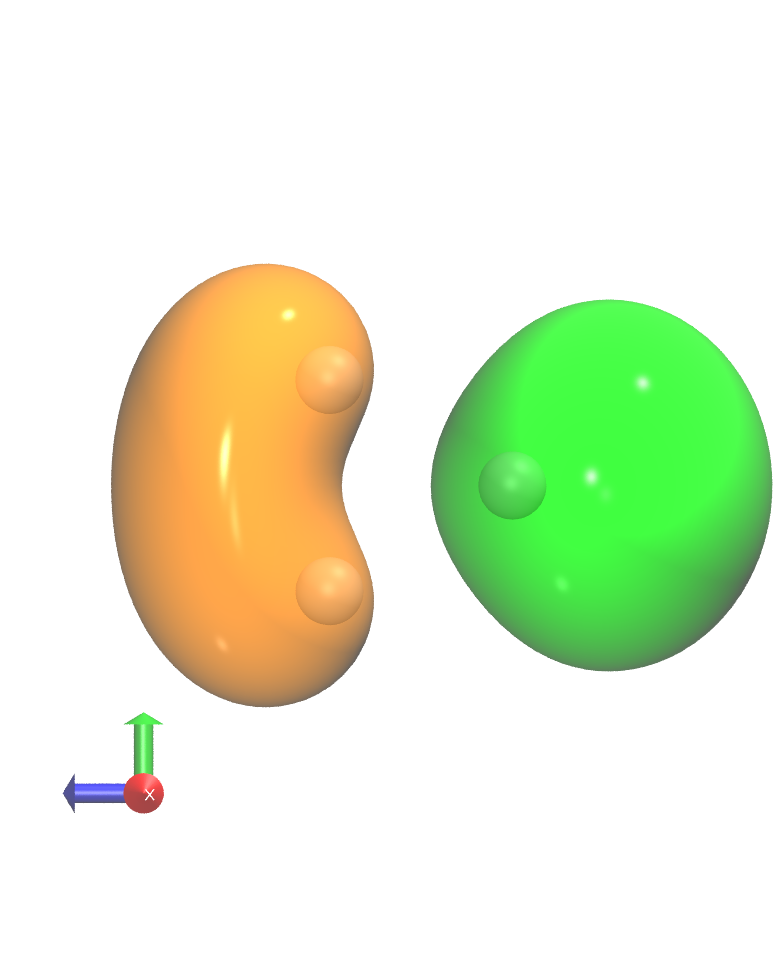
\includegraphics{./cursym/data/h3/b2_1200ppi.png}}
            \end{subfigure}
            \unskip\ \vrule\
            \begin{subfigure}{.40\textwidth}
              \centering
              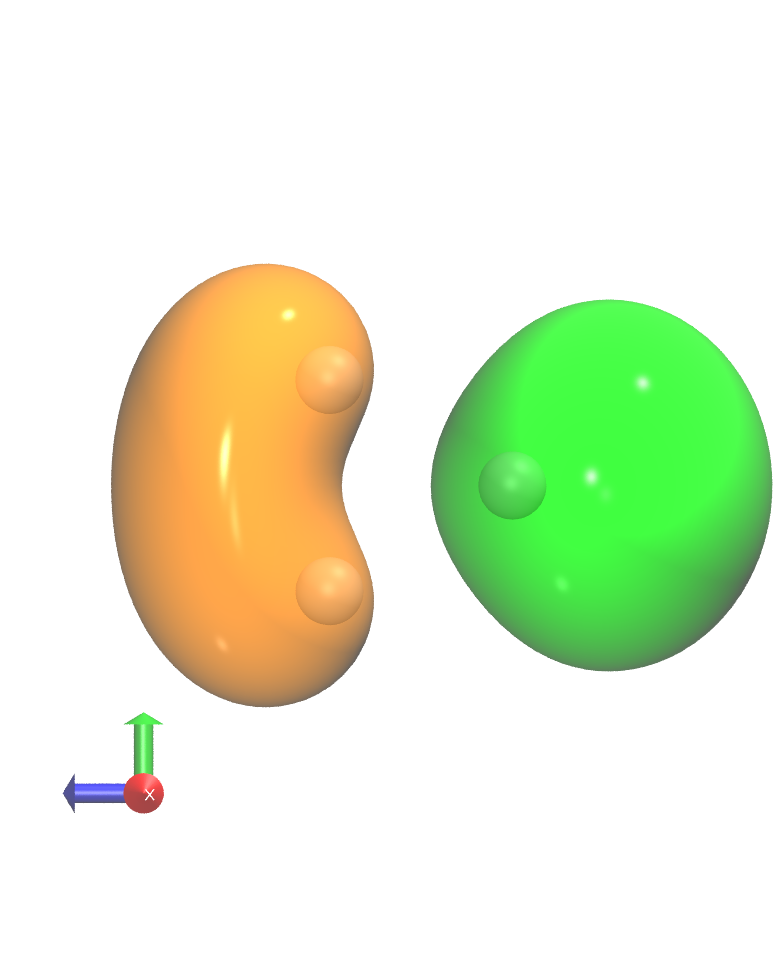
\includegraphics{./cursym/data/h3/b2_1200ppi.png}
              \subcaption{$\beta_2$, $A'_1 \oplus E' (\symcal{D}_{3h})$}
            \end{subfigure}

            \begin{subfigure}{.40\textwidth}
              \centering
              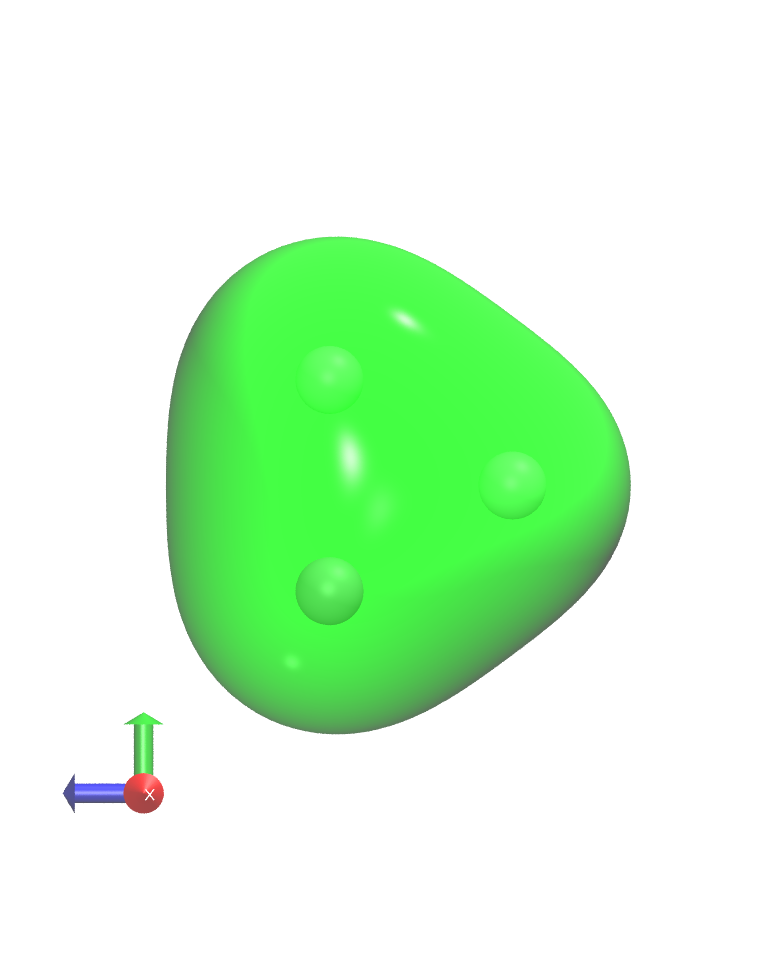
\includegraphics{./cursym/data/h3/a1_1200ppi.png}
              \subcaption{$\alpha_1$, $A'_1 \oplus E' (\symcal{D}_{3h})$}
            \end{subfigure}
            \unskip\ \vrule\
            \begin{subfigure}{.40\textwidth}
              \centering
              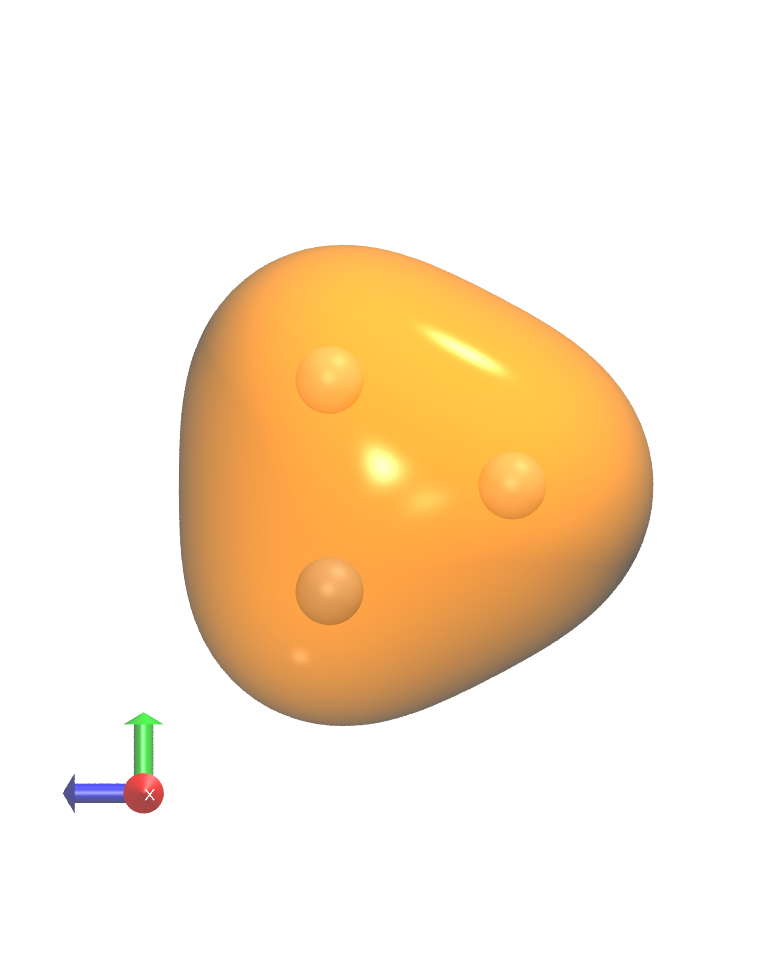
\includegraphics{./cursym/data/h3/b1_1200ppi.png}
              \subcaption{$\beta_1$, $A'_1 \oplus E' (\symcal{D}_{3h})$}
            \end{subfigure}
          \end{figure}
        \end{itemize}
      }

      \only<4->{
        \item<4-> This \glsxtrshort*{acr:uhf} symmetry breaking \emphit{Magenta}{persists} at finite field strengths:
        \begin{figure}
          \centering
          \pgfplotstableread[col sep=comma]{cursym/data/h3/h3.t60.000.csv}\data

\begin{tikzpicture}[%
]
  % Main plot
  \begin{groupplot}[
    % =============
    % Group configs
    % =============
    group style={
      group size=1 by 1,
      xlabels at=edge bottom,
      xticklabels at=edge bottom,
      ylabels at=edge left,
      yticklabels at=edge left,
      vertical sep=1.5cm,
      horizontal sep=1.8cm,
    },
    % =================
    % Groupplot general
    % =================
    width=.5\linewidth,
    scale only axis=true,
    cycle list name=coloronly,
    unbounded coords=jump,
    % ==================
    % Group title format
    % ==================
    title style={yshift=-1.5ex, font={\footnotesize}},
    % =================
    % Group axis format
    % =================
    % -----------------
    % Group axis scales
    % -----------------
    xmin=0, xmax=1,
    ymin=-1.725, ymax=-1.45,
    % -----------------
    % Group axis labels
    % -----------------
    xlabel={$\lvert \gls*{mag:vec} \rvert / B_0$},
    label style={font=\scriptsize},
    xlabel style={align=center},
    every axis y label/.append style={at={(0, 0.5)}, yshift=2.5em},
    % -----------------
    % Group tick labels
    % -----------------
    tick label style={font=\scriptsize},
    x tick label style=
    {
      /pgf/number format/.cd,
      fixed,
      fixed zerofill,
      precision=1,
      /tikz/.cd
    },
%    every y tick scale label/.style={%
%      at={(yticklabel cs:1)},%
%      anchor=east,%
%      inner sep=1pt%
%    },
    % ------------------
    % Group tick configs
    % ------------------
    xtick pos=left,
    xtick align=outside,
    minor x tick num=1,
    xtick distance=0.2,
    %%%%%%%%%%%%%%%%%%%%%%%%%%%%%
  ]
    % ==
    % ==
    % Wc
    % ==
    % ==
    % ------
    % Carbon
    % ------
    \nextgroupplot[
      % ===============
      % Subplot general
      % ===============
      align=center,
      ylabel={UHF energy / \si{\hartree}},
      height=.6\textheight,
      % ====================
      % Subplot title format
      % ====================
      % ===================
      % Subplot axis format
      % ===================
      % -------------------
      % Subplot axis scales
      % -------------------
      % -------------------
      % Subplot axis labels
      % -------------------
      y tick label style=
      {
        /pgf/number format/.cd,
        fixed,
        fixed zerofill,
        precision=2,
        /tikz/.cd
      },
      % -------------------
      % Subplot tick labels
      % -------------------
      % --------------------
      % Subplot tick configs
      % --------------------
      ytick align=outside,
      ytick pos=left,
      minor y tick num=1,
%      ytick distance=0.05,
      % ===============
      % Subplot legends
      % ===============
      legend pos=north east,
      legend style={
        legend cell align=right,
        legend style={font=\scriptsize},
      },
      % ===================
      % Subplot annotations
      % ===================
      after end axis/.code={%
        % ============
        % Point groups
        % ============
        \draw[<-, very thin] (rel axis cs:0, 1.015) -- ++(axis direction cs:0, 0.01) node[anchor=south, scale=0.5, inner sep=2pt] {$\symcal{D}_{3h}$};
        \node[anchor=south, scale=0.5, inner sep=2pt] at (rel axis cs:0.5, 1.020) {$\symcal{C}_{3h}$};
        % ===============
        % Symmetry labels
        % ===============
        \pgfplotstablegetelem{0}{s0_sym0_energy}\of{\data}
        \draw[very thin, ->] (axis cs:0, \pgfplotsretval) -- ++(axis direction cs:0.15, 0.01) node[anchor=west, scale=0.7, inner sep=2pt] {$A'_1 \oplus E' (\symcal{D}_{3h})$};
        \pgfplotstablegetelem{5}{s0_sym0_energy}\of{\data}
        \draw[very thin, ->] (axis cs:0.25, \pgfplotsretval) -- ++(axis direction cs:0.10, 0.025) node[anchor=south west, scale=0.7, inner sep=2pt] {$A' \oplus \Gamma' \oplus \bar{\Gamma}' (\symcal{C}_{3h})$};
      },
    ]
      \addplot[%
        DarkGreen,%
        smooth,
        very thick,%
        mark=none,%
      ] table[x={bx}, y={s0_sym0_energy}]{\data};
      \addlegendentry{$\gls*{wf:uhf}$}
      \addplot[%
        blue,%
        only marks,%
        mark=x,%
        mark size=2pt,%
      ] table[x={bx}, y={s0_sym1_energy}]{\data};
      \addlegendentry{$\hat{C}_3 \gls*{wf:uhf}$}
      \addplot[%
        red,%
        only marks,%
        mark=o,%
        mark size=1.5pt,%
      ] table[x={bx}, y={s0_sym2_energy}]{\data};
      \addlegendentry{$\hat{C}_3^{-1} \gls*{wf:uhf}$}
  \end{groupplot}
\end{tikzpicture}
        \end{figure}
      }
    \end{itemize}
  \end{frame}


  \subsection{\ce{H6} octahedron}
  %%%%%%%%%%%%%%%%%%%%%%%%%%
  %%%%%%%%%%%%%%%%%%%%%%%%%%
  \begin{frame}{Degenerate current density symmetry}
    \begin{itemize}
      \item<1-> Consider an octahedral \ce{H6} cluster.
      \begin{figure}
        \centering
        \scalebox{.8}{\ifdefined\molsize
  \setlength{\molsize}{1.2cm}
\else
  \newlength{\molsize}
  \setlength{\molsize}{1.2cm}
\fi
\begin{tikzpicture}
  \coordinate (top) at (0, 0.50\molsize);
  \coordinate (bottom) at (0, -0.50\molsize);
  \coordinate (topleft) at (-0.553\molsize, 0.242\molsize);
  \coordinate (bottomleft) at (-0.553\molsize, -0.242\molsize);
  \coordinate (topright) at (0.553\molsize, 0.242\molsize);
  \coordinate (bottomright) at (0.553\molsize, -0.242\molsize);
  % =====================
  % Molecular arrangement
  % =====================
  \draw[densely dotted] (top) -- (bottom);
  \draw[densely dotted] (topleft) -- (bottomright);
  \draw[densely dotted] (topright) -- (bottomleft);
  \node[draw, shape=circle, fill=gray, scale=0.4] at (top) {};
  \node[draw, shape=circle, fill=gray, scale=0.4] at (bottom) {};
  \node[draw, shape=circle, fill=gray, scale=0.4] at (topleft) {};
  \node[draw, shape=circle, fill=gray, scale=0.4] at (bottomleft) {};
  \node[draw, shape=circle, fill=gray, scale=0.4] at (topright) {};
  \node[draw, shape=circle, fill=gray, scale=0.4] at (bottomright) {};
  % =====
  % Field
  % =====
  \draw[->, very thick] (2, 0) -- ++(0, 0.7) node[scale=0.6, anchor=south, inner sep=1pt] {$\symbfit{B}$};
  % =================
  % Coordinate system
  % =================
  \draw[->] (3, 0) -- ++(0.553, -0.242) node[anchor=west, scale=0.7] {$y$};
  \draw[->] (3, 0) -- ++(0, 0.7) node[anchor=south, scale=0.7] {$z$};
  \draw[->] (3, 0) -- ++(-0.553, -0.242) node[anchor=north east, scale=0.7] {$x$};
\end{tikzpicture}}
      \end{figure}

      \item<1-> Back-of-the-envelope properties for $\gls*{mag:vec}$ along $z$:
      \begin{columns}[T]
        \begin{column}{.40\textwidth}
          \emphbf{red}{Zero field}
          \begin{itemize}
            \item<1-> Spatial sym. group: $\symcal{G} = \textcolor{red}{\symcal{O}_{h}}$
          \end{itemize}
        \end{column}
        \begin{column}{.50\textwidth}
          \emphbf{blue}{Finite fields}
          \begin{itemize}
            \item<1-> Magnetic sym. group: $\symcal{M} = \textcolor{blue}{\symcal{D}_{4h}(\symcal{C}_{4h})}$
            \begin{itemize}
              \item Mag. unitary sym. subgroup: $\symcal{H} = \symcal{C}_{4h}$
              \item Spatial pseudo-sym. group: $\symcal{G} = \symcal{O}_{h}$
            \end{itemize}
          \end{itemize}
        \end{column}
      \end{columns}

      \vspace{6pt}

      \begin{columns}[T]
        \begin{column}{.40\textwidth}
        \end{column}
        \begin{column}{.50\textwidth}
          \begin{itemize}
            \item<1-> Ground current: $\textcolor{blue}{A_g(\symcal{C}_{4h})} \leftarrow \textcolor{red}{T_{1g}(\symcal{O}_{h})}$
          \end{itemize}
        \end{column}
      \end{columns}
    \end{itemize}
  \end{frame}


  %%%%%%%%%%%%%%%%%%%%%%%%%%
  %%%%%%%%%%%%%%%%%%%%%%%%%%
  \begin{frame}{Principal-field current density in \ce{H6} cluster}
    \begin{columns}
      \begin{column}{.40\textwidth}
        \begin{itemize}
          \setlength\itemsep{1.2em}
          \item<1-> \glsxtrshort*{acr:uhf}, 6-31G*, $M_S = 0$
          \item<1-> $\gls*{mag:vec}$ along $z$-direction
          \item<1-> $\gls*{mag:jphys}(\gls*{bas:spatialcoord})$ symmetry: $\textcolor{blue}{A_g(\symcal{C}_{4h})} \leftarrow \textcolor{red}{T_{1g}(\symcal{O}_{h})}$
          \item<1-> \glsxtrshort*{acr:uhf} symmetry: $B_g(\symcal{C}_{4h})$
        \end{itemize}
      \end{column}

      \begin{column}{.55\textwidth}
        \begin{figure}
          \centering
          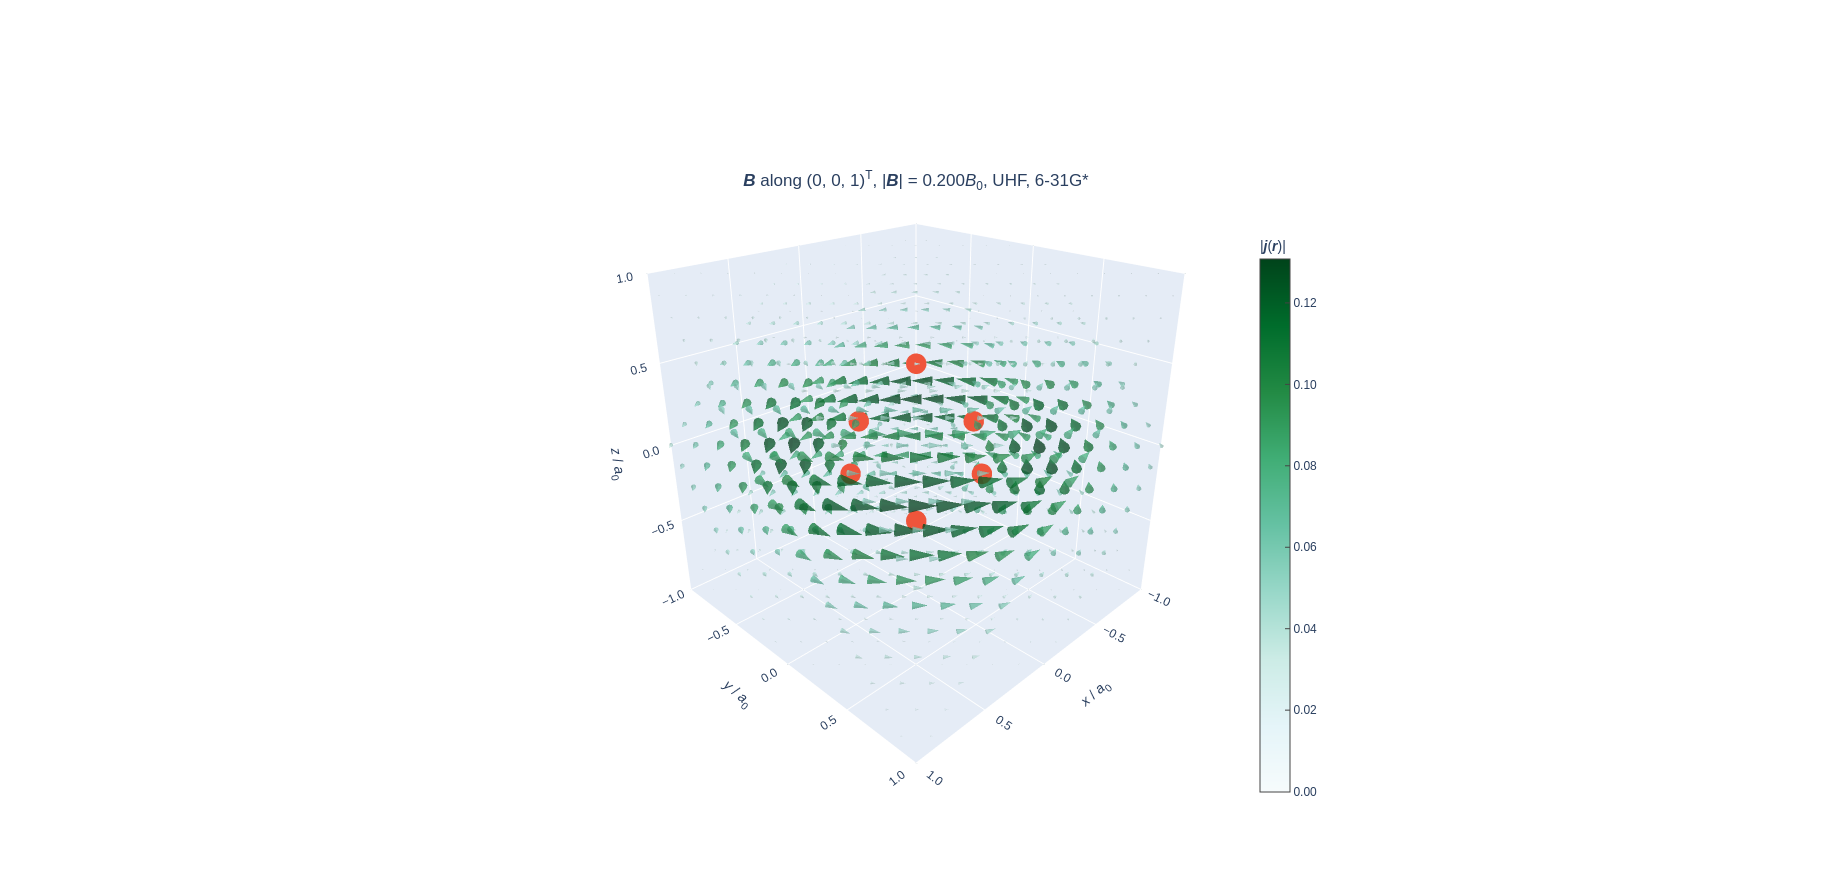
\includegraphics[trim=600 50 500 150, clip, width=\textwidth]{./cursym/data/h6/bz.png}
        \end{figure}
      \end{column}
    \end{columns}
  \end{frame}


  %%%%%%%%%%%%%%%%%%%%%%%%%%
  %%%%%%%%%%%%%%%%%%%%%%%%%%
  \begin{frame}{Non-principal-field current density in \ce{H6} cluster}
    \begin{columns}
      \begin{column}{.40\textwidth}
        \begin{itemize}
          \setlength\itemsep{1.2em}
          \item<1-> \glsxtrshort*{acr:uhf}, 6-31G*, $M_S = 0$
          \item<1-> $\gls*{mag:vec}$ along $(1, 1, 1)^{\T}$ direction
          \item<1-> $\gls*{mag:jphys}(\gls*{bas:spatialcoord})$ symmetry: $\textcolor{blue}{A_g(\symcal{S}_{6})} \leftarrow \textcolor{red}{\underline{T_{1g}} \oplus A_{2g}(\symcal{O}_{h})}$
          \item<1-> \glsxtrshort*{acr:uhf} symmetry: $\bar{\Gamma}_g(\symcal{S}_{6})$
        \end{itemize}
      \end{column}

      \begin{column}{.55\textwidth}
        \begin{figure}
          \centering
          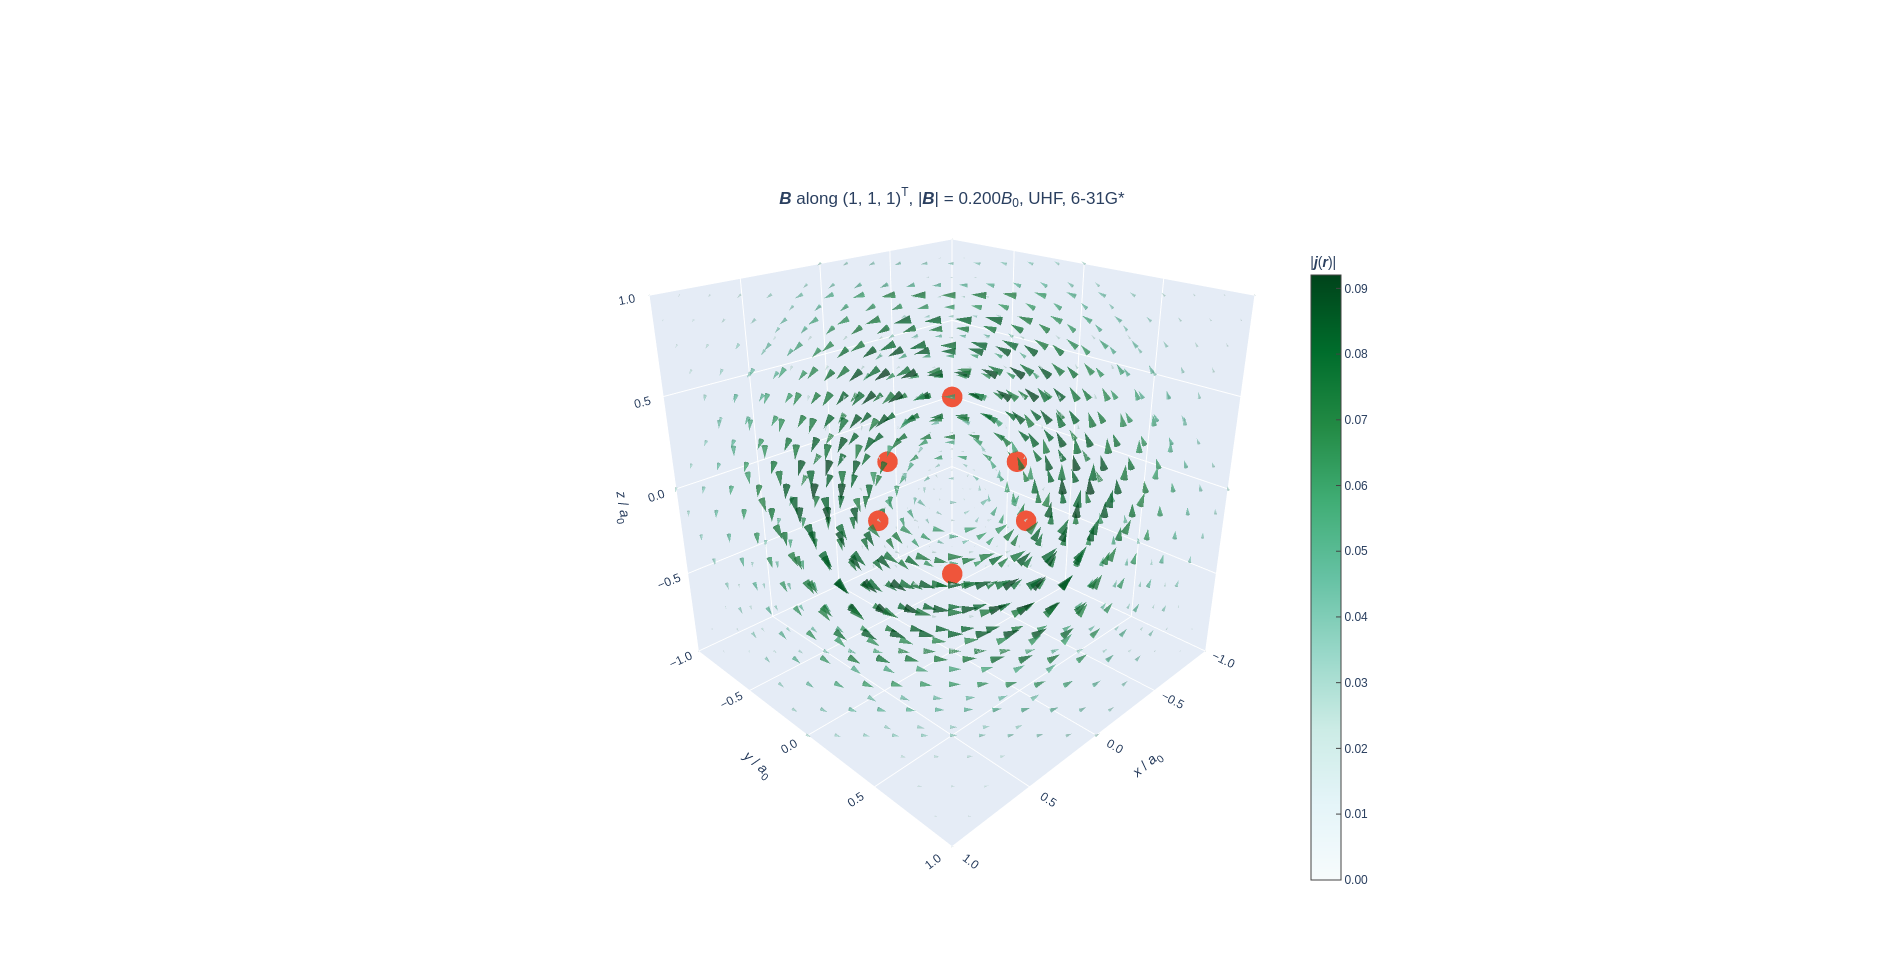
\includegraphics[trim=600 50 500 150, clip, width=\textwidth]{./cursym/data/h6/bxyz.png}
        \end{figure}
      \end{column}
    \end{columns}
  \end{frame}
  \section{\$}
%%%%%%%%%%%%%%%%%%%%%%%%%%
%%%%%%%%%%%%%%%%%%%%%%%%%%
\begin{frame}{Conclusion and Outlook}
  \begin{itemize}
    \item Completed:
    \begin{itemize}
      \item Developed a \emphit{Magenta}{unitary}-symmetry-based framework to characterise the \emphit{Magenta}{spatial} properties of magnetically induced current densities
      \item Tested the framework on simple, high-symmetry systems
    \end{itemize}

    \item To do:
    \begin{itemize}
      \item Relate the unitary symmetry of current densities to other magnetic properties calculated from them
      \item Extend the framework to \emphbf{DarkGreen}{corepresentations} to take into account \emphit{Magenta}{antiunitary} symmetry
      \item Consider also \emphbf{DarkGreen}{double-valued} representations and corepresentations to handle odd-electron systems correctly
    \end{itemize}
  \end{itemize}
\end{frame}


%%%%%%%%%%%%%%%%%%%%%%%%%%%%%%%%%%%%%%%%%%%%%%%%%%%%%%%
%%%%%%%%%%%%%%%%%%%%%%%%%%%%%%%%%%%%%%%%%%%%%%%%%%%%%%%
\subsection{Acknowledgements}
\begin{frame}{Acknowledgements}
  \begin{itemize}
    \item Prof. Andy Teale for magnetism and current discussions
    \item Dr Tom Irons for symmetry and integral discussions
    \item The rest of Teale group for general support
  \end{itemize}
\end{frame}


\end{document}